%%%%%%%%%%%%%%%%%%%%%%%%%%%%%%%%%%%%%%%%%
% Jacobs Landscape Poster
% LaTeX Template
% Version 1.1 (14/06/14)
%
% Created by:
% Computational Physics and Biophysics Group, Jacobs University
% https://teamwork.jacobs-university.de:8443/confluence/display/CoPandBiG/LaTeX+Poster
% 
% Further modified by:
% Nathaniel Johnston (nathaniel@njohnston.ca)
%
% This template has been downloaded from:
% http://www.LaTeXTemplates.com
%
% License:
% CC BY-NC-SA 3.0 (http://creativecommons.org/licenses/by-nc-sa/3.0/)
%
%%%%%%%%%%%%%%%%%%%%%%%%%%%%%%%%%%%%%%%%%

%----------------------------------------------------------------------------------------
%	PACKAGES AND OTHER DOCUMENT CONFIGURATIONS
%----------------------------------------------------------------------------------------

\documentclass[final]{beamer}

\usepackage[scale=1.24]{beamerposter} % Use the beamerposter package for laying out the poster

\usetheme{confposter} % Use the confposter theme supplied with this template

\setbeamercolor{block title}{fg=ngreen,bg=white} % Colors of the block titles
\setbeamercolor{block body}{fg=black,bg=white} % Colors of the body of blocks
\setbeamercolor{block alerted title}{fg=white,bg=dblue!70} % Colors of the highlighted block titles
\setbeamercolor{block alerted body}{fg=black,bg=dblue!10} % Colors of the body of highlighted blocks
% Many more colors are available for use in beamerthemeconfposter.sty

%-----------------------------------------------------------
% Define the column widths and overall poster size
% To set effective sepwid, onecolwid and twocolwid values, first choose how many columns you want and how much separation you want between columns
% In this template, the separation width chosen is 0.024 of the paper width and a 4-column layout
% onecolwid should therefore be (1-(# of columns+1)*sepwid)/# of columns e.g. (1-(4+1)*0.024)/4 = 0.22
% Set twocolwid to be (2*onecolwid)+sepwid = 0.464
% Set threecolwid to be (3*onecolwid)+2*sepwid = 0.708

\newlength{\sepwid}
\newlength{\onecolwid}
\newlength{\twocolwid}
\newlength{\threecolwid}
\setlength{\paperwidth}{48in} % A0 width: 46.8in
\setlength{\paperheight}{36in} % A0 height: 33.1in
\setlength{\sepwid}{0.024\paperwidth} % Separation width (white space) between columns
\setlength{\onecolwid}{0.22\paperwidth} % Width of one column
\setlength{\twocolwid}{0.464\paperwidth} % Width of two columns
\setlength{\threecolwid}{0.708\paperwidth} % Width of three columns
\setlength{\topmargin}{-0.5in} % Reduce the top margin size
%-----------------------------------------------------------

\usepackage{graphicx}  % Required for including images

\usepackage{booktabs} % Top and bottom rules for tables

\usepackage{fontawesome} % logo

\usepackage{verbatim}

%----------------------------------------------------------------------------------------
%	TITLE SECTION 
%----------------------------------------------------------------------------------------

\title{The Pipeline of Data Visualization \\ {\LARGE illustrated with Swiss parliament data}} % Poster title

\author{Joachim Muth, Gael Lederrey \& Jonas Racine} % Author(s)

\institute{\'Ecole Polytechnique F\'ed\'erale de Lausanne} % Institution(s)



%----------------------------------------------------------------------------------------

\begin{document}

\addtobeamertemplate{headline}{} 
{
\begin{tikzpicture}[remember picture,overlay] 
\node [shift={(-16.4 cm,-6cm)}] at (current page.north east) {
\includegraphics[height=7cm]{img/ada_logo} ~ ~ ~ ~ ~ ~ 
\includegraphics[height=7cm]{img/epfl_logo}}; 
\end{tikzpicture} 
\begin{tikzpicture}[remember picture,overlay] 
\node [shift={(10cm,-6cm)}] at (current page.north west) {
\includegraphics[height=7cm]{img/parlament_logo}}; 
\end{tikzpicture} 
}


\addtobeamertemplate{block end}{}{\vspace*{2ex}} % White space under blocks
\addtobeamertemplate{block alerted end}{}{\vspace*{2ex}} % White space under highlighted (alert) blocks

\setlength{\belowcaptionskip}{2ex} % White space under figures
\setlength\belowdisplayshortskip{2ex} % White space under equations

\setbeamercolor{block title}{fg=MidnightBlue,bg=white} % Change the block title color

\begin{frame}[t] % The whole poster is enclosed in one beamer frame

\begin{columns}[t] % The whole poster consists of three major columns, the second of which is split into two columns twice - the [t] option aligns each column's content to the top

\begin{column}{\sepwid}\end{column} % Empty spacer column

\begin{column}{\onecolwid} % The first column

%----------------------------------------------------------------------------------------
%	INTRO
%----------------------------------------------------------------------------------------

\begin{block}{Introduction}

This project represents the final point of {\bf Applied Data Analysis} course, taught by Michele Catasta in 2016. We put into practice the analysis of real-world data, following the whole pipeline from {\bf scraping} to {\bf interactive visualization}. By doing so we experienced the \textbf{real-world challenges} that arise in such a project. Our case study focuses on the data available on \url{hwww.parliament.ch}.

\end{block}

%----------------------------------------------------------------------------------------
%	MOTIVATION
%----------------------------------------------------------------------------------------

\begin{block}{Motivation}

Since the \textbf{Freedom of Information Act} entered into force (on 1 July 2006) a huge amount of data related to political activities is freely available to the public. However, it represents a large number of hardly understandable documents. We suggest an interface giving a \textbf{light overview} of Swiss parliamentary activities.

\end{block}

%----------------------------------------------------------------------------------------
%	1. ACQUISITION
%----------------------------------------------------------------------------------------

\begin{alertblock}{1. Data Acquisition}

Parliament IT service provides an API which allows direct access to database tables. However, it presents some restrictions:

\begin{itemize}
\item \textbf{Limited} number of returned items per request
\item A \textbf{timeout} so short it makes it impossible to use \texttt{skip} to access last elements of big tables.
\end{itemize}

To overcome these issues we developed a Python scraper that bypasses these restrictions.

\end{alertblock}

%----------------------------------------------------------------------------------------
%	2. Cleaning
%----------------------------------------------------------------------------------------

\begin{alertblock}{2. Data Preparation \& Cleaning}

The database tables collected contain numerous problems:
\begin{itemize}
\item Hashed primary key (ID)
\item Multiple entries for same item in different languages
\item 3 different IDs to designate a member of parliament
\end{itemize}

\end{alertblock}



%------------------------------------------------

%\begin{figure}
%
\includegraphics[width=0.8\linewidth]{placeholder.jpg}
%\caption{Figure caption}
%\end{figure}

%----------------------------------------------------------------------------------------

\end{column} % End of the first column

\begin{column}{\sepwid}\end{column} % Empty spacer column

\begin{column}{\twocolwid} % Begin a column which is two columns wide (column 2)

\begin{columns}[t,totalwidth=\twocolwid] % Split up the two columns wide column

\begin{column}{\onecolwid}\vspace{-.6in} % The first column within column 2 (column 2.1)


%----------------------------------------------------------------------------------------
%	3. RESTRICTION
%----------------------------------------------------------------------------------------

\begin{alertblock}{3. Constraints}

As we are working on data involving public people, we refrain from any \textbf{subjective interpretation}. Instead, we focus on a visualization tool that other people (e.g. journalists) can use to draw conclusions. Hence, it needed to be transparent enough to be trusted.

\end{alertblock}


%----------------------------------------------------------------------------------------

\end{column} % End of column 2.1

\begin{column}{\onecolwid}\vspace{-.6in} % The second column within column 2 (column 2.2)


%----------------------------------------------------------------------------------------
%	4. INTERPRETATION
%----------------------------------------------------------------------------------------

\begin{alertblock}{4. Data Interpretation}

Under reasonable assumptions:
\begin{itemize}
\item \textbf{Involvement:} number of speeches and initiatives
\item \textbf{Interests:} distribution of written and signed initiatives among themes.
\item \textbf{Partnerships:} cosigned initiatives.
\end{itemize}

\end{alertblock}

%----------------------------------------------------------------------------------------

\end{column} % End of column 2.2

\end{columns} % End of the split of column 2 - any content after this will now take up 2 columns width

%----------------------------------------------------------------------------------------
%	CENTRAL PICTURE
%----------------------------------------------------------------------------------------

\begin{center}
\begin{tabular}{ccc}
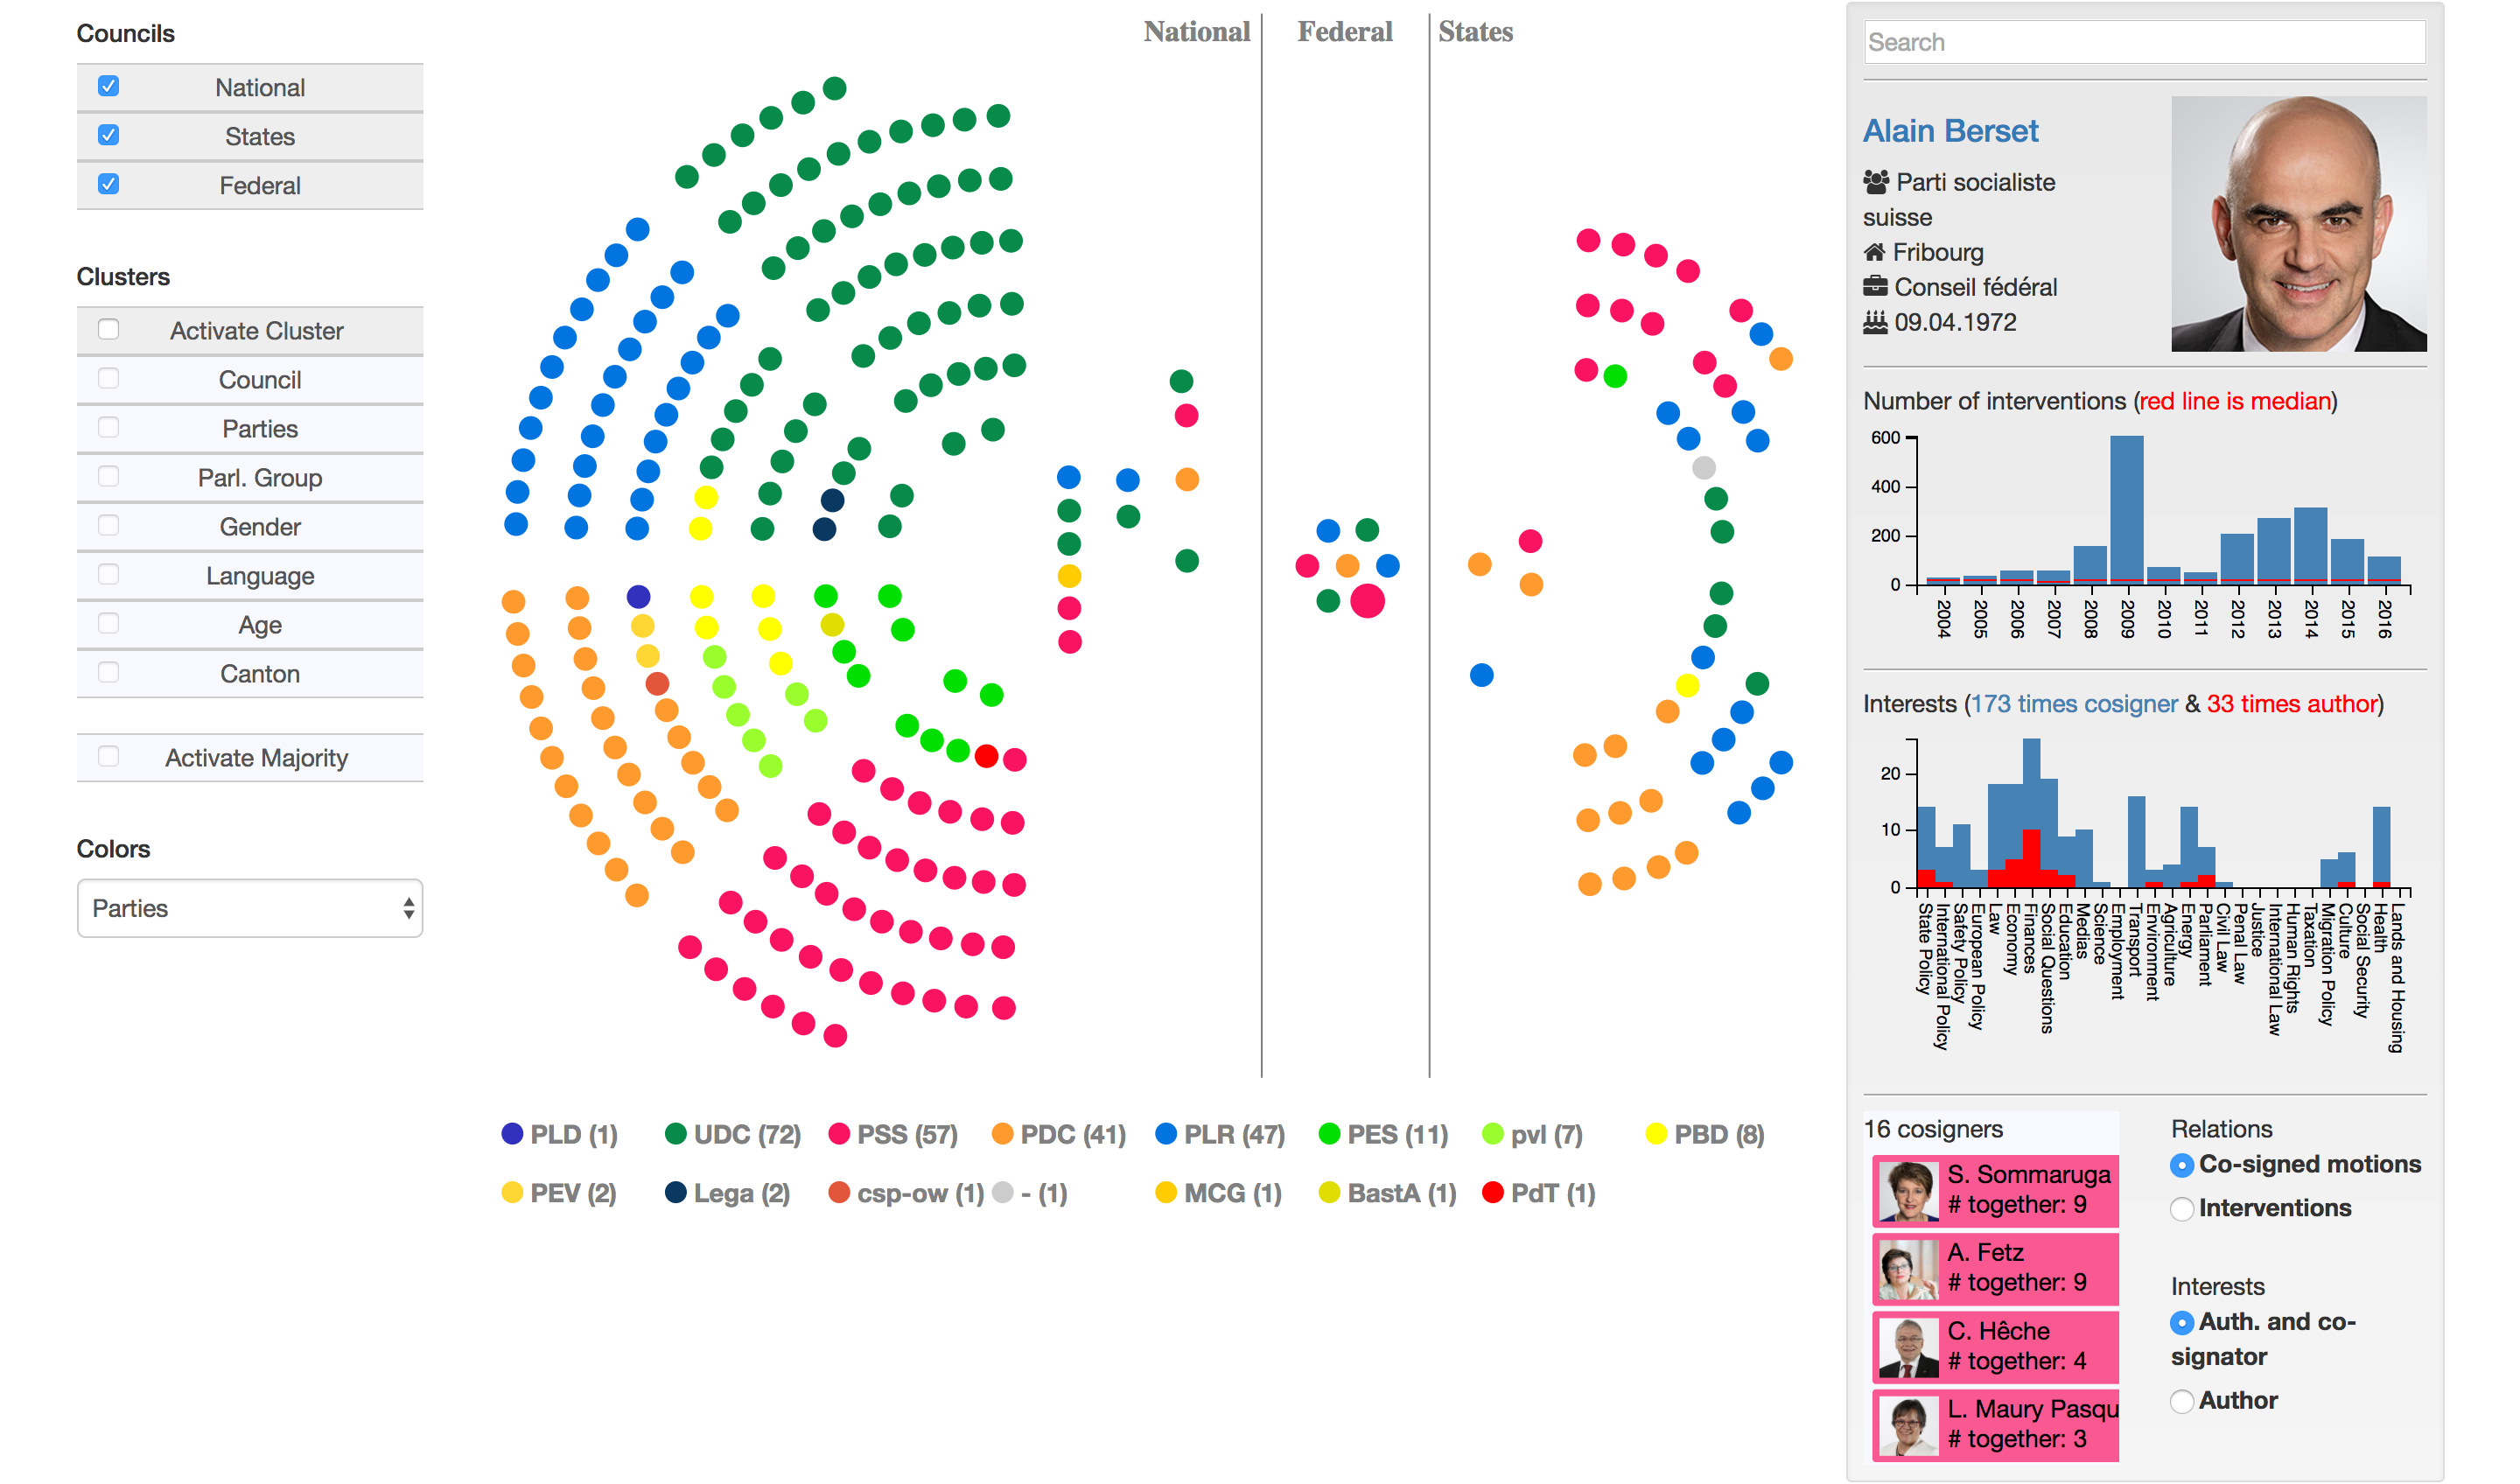
\includegraphics[width=1\linewidth]{img/capture_no_border}
\end{tabular}
\end{center}

%
%\begin{alertblock}{Important Result}
%
%Lorem ipsum dolor \textbf{sit amet}, consectetur adipiscing elit. Sed commodo molestie porta. Sed ultrices scelerisque sapien ac commodo. Donec ut volutpat elit.
%
%\end{alertblock} 

%----------------------------------------------------------------------------------------

\begin{columns}[t,totalwidth=\twocolwid] % Split up the two columns wide column again

\begin{column}{\onecolwid} % The first column within column 2 (column 2.1)

%----------------------------------------------------------------------------------------
%	CONCLUSION
%----------------------------------------------------------------------------------------

\begin{block}{Conclusion}

This project gives an \textbf{overview of some challenges} that can be encountered at each step of the process when trying to analyse real-world data. It highlights the interdisciplinarity of data analysis, requiring the full range of skills: \textbf{coding} to master the numerous IT tools; \textbf{analytical} to decide what to focus on; \textbf{curiosity} to understand the field the data come from; \textbf{social} to interact with domain experts and understand their point of view.

\end{block}

%----------------------------------------------------------------------------------------

\end{column} % End of column 2.1

\begin{column}{\onecolwid} % The second column within column 2 (column 2.2)

%----------------------------------------------------------------------------------------
%	OTHER
%----------------------------------------------------------------------------------------

\begin{block}{Involved IT tools}

\begin{itemize}
\item Scraping and data analysis with \textbf{Python}, enhanced with Pandas, NumPy and SciPy libraries.
\item Visualization with \textbf{JavaScript}, enhanced with D3.js and JQuery
\item Website design with \textbf{Bootstrap}.
\end{itemize}


%
%\begin{figure}
%
\includegraphics[width=0.8\linewidth]{placeholder.jpg}
%\caption{Figure caption}
%\end{figure}

\end{block}

%----------------------------------------------------------------------------------------

\end{column} % End of column 2.2

\end{columns} % End of the split of column 2

\end{column} % End of the second column

\begin{column}{\sepwid}\end{column} % Empty spacer column

\begin{column}{\onecolwid} % The third column

%----------------------------------------------------------------------------------------
%	5. VISUALIZATION
%----------------------------------------------------------------------------------------

\begin{alertblock}{5. Visualization}

We want the visualization to be: 
\begin{itemize}
\item \textbf{Intuitive} enough to be used without explanation.
\item \textbf{Enjoyable}, so people have fun exploring it.
\item \textbf{Single-Page}, to lower complexity
\item Focused on the \textbf{individuals} or \textbf{agglomerated groups}.
\end{itemize}


\end{alertblock}

%----------------------------------------------------------------------------------------
%	6. DOMAIN EXPERT
%----------------------------------------------------------------------------------------

\begin{alertblock}{6. Assessment from Domain Experts}

Meeting with \textbf{Alain Rebetez}, political journalist, and \textbf{Philippe Nantermod}, PLR deputy.

\begin{itemize}
\item Expertise about the political system.
\item Is the visualization intuitive enough?
\item What information would they like to see?
\end{itemize}



\end{alertblock}

%----------------------------------------------------------------------------------------
%	... and next ?
%----------------------------------------------------------------------------------------

\begin{alertblock}{7. ... and next ?}

Go back to point 4 and iterate until reaching the deadline :)

\end{alertblock}

%%----------------------------------------------------------------------------------------
%%	REFERENCES
%%----------------------------------------------------------------------------------------
%
%\begin{block}{References}
%
%\nocite{*} % Insert publications even if they are not cited in the poster
%\small{\bibliographystyle{unsrt}
%\bibliography{sample}\vspace{0.75in}}
%
%\end{block}

%----------------------------------------------------------------------------------------
%	ACKNOWLEDGEMENTS
%----------------------------------------------------------------------------------------

\begin{block}{Acknowledgements}

\small{\rmfamily{A warm thank you to \textbf{Alain Rebetez}, political journalist, \textbf{Philippe Nantermod}, PLR deputy, and \textbf{Mathias Reynard}, PS deputy, for their expertise in the Swiss parliamentary system, their advice and their external point of view on the project.}} \\

\end{block}

%----------------------------------------------------------------------------------------
%	CONTACT INFORMATION
%----------------------------------------------------------------------------------------

\setbeamercolor{block alerted title}{fg=black,bg=norange} % Change the alert block title colors
\setbeamercolor{block alerted body}{fg=black,bg=white} % Change the alert block body colors

\begin{alertblock}{Contact Information}

\begin{itemize}
\item[] \faGithub ~ \href{https://github.com/jmuth/parliament-viz.ch}{github.com/jmuth/parliament-viz.ch}
\item[] \faGlobe ~ \href{http://parliament-viz.ch}{www.parliament-viz.ch}
\item[] \faAt ~ \href{mailto:joachim.muth@epfl.ch}{joachim.muth@epfl.ch} \\ ~ ~ \,\href{mailto:gael.lederrey@epfl.ch}{gael.lederrey@epfl.ch} \\ ~ ~ \,\href{mailto:jonas.racine@epfl.ch}{jonas.racine@epfl.ch}

\end{itemize}

\end{alertblock}

%\begin{center}
%\begin{tabular}{ccc}
%
\includegraphics[width=0.4\linewidth]{logo.png} & \hfill & 
\includegraphics[width=0.4\linewidth]{logo.png}
%\end{tabular}
%\end{center}

%----------------------------------------------------------------------------------------

\end{column} % End of the third column

\end{columns} % End of all the columns in the poster

\end{frame} % End of the enclosing frame

\end{document}
